\documentclass[tikz]{standalone}
%\usepackage{pgfplots}
%\pgfplotsset{compat=1.11}

\definecolor{Set1-7-1}{RGB}{228,26,28}
\definecolor{Set1-7-2}{RGB}{55,126,184}
\definecolor{Set1-7-3}{RGB}{77,175,74}
\definecolor{Set1-7-4}{RGB}{152,78,163}
\definecolor{Set1-7-5}{RGB}{255,127,0}
\definecolor{Set1-7-6}{RGB}{255,255,51}
\definecolor{Set1-7-7}{RGB}{166,86,40}

\usepackage{mathspec}
\setromanfont[Numbers={Lining,Proportional}]{Minion Pro}
\setmathsfont(Digits,Latin,Greek)[Numbers={Lining,Proportional}]{Minion Pro}
\setmathrm{Minion Pro}
\usepackage{fix-cm}
\begin{document}
\begin{tikzpicture}[level/.style={thick}]
\pgftext{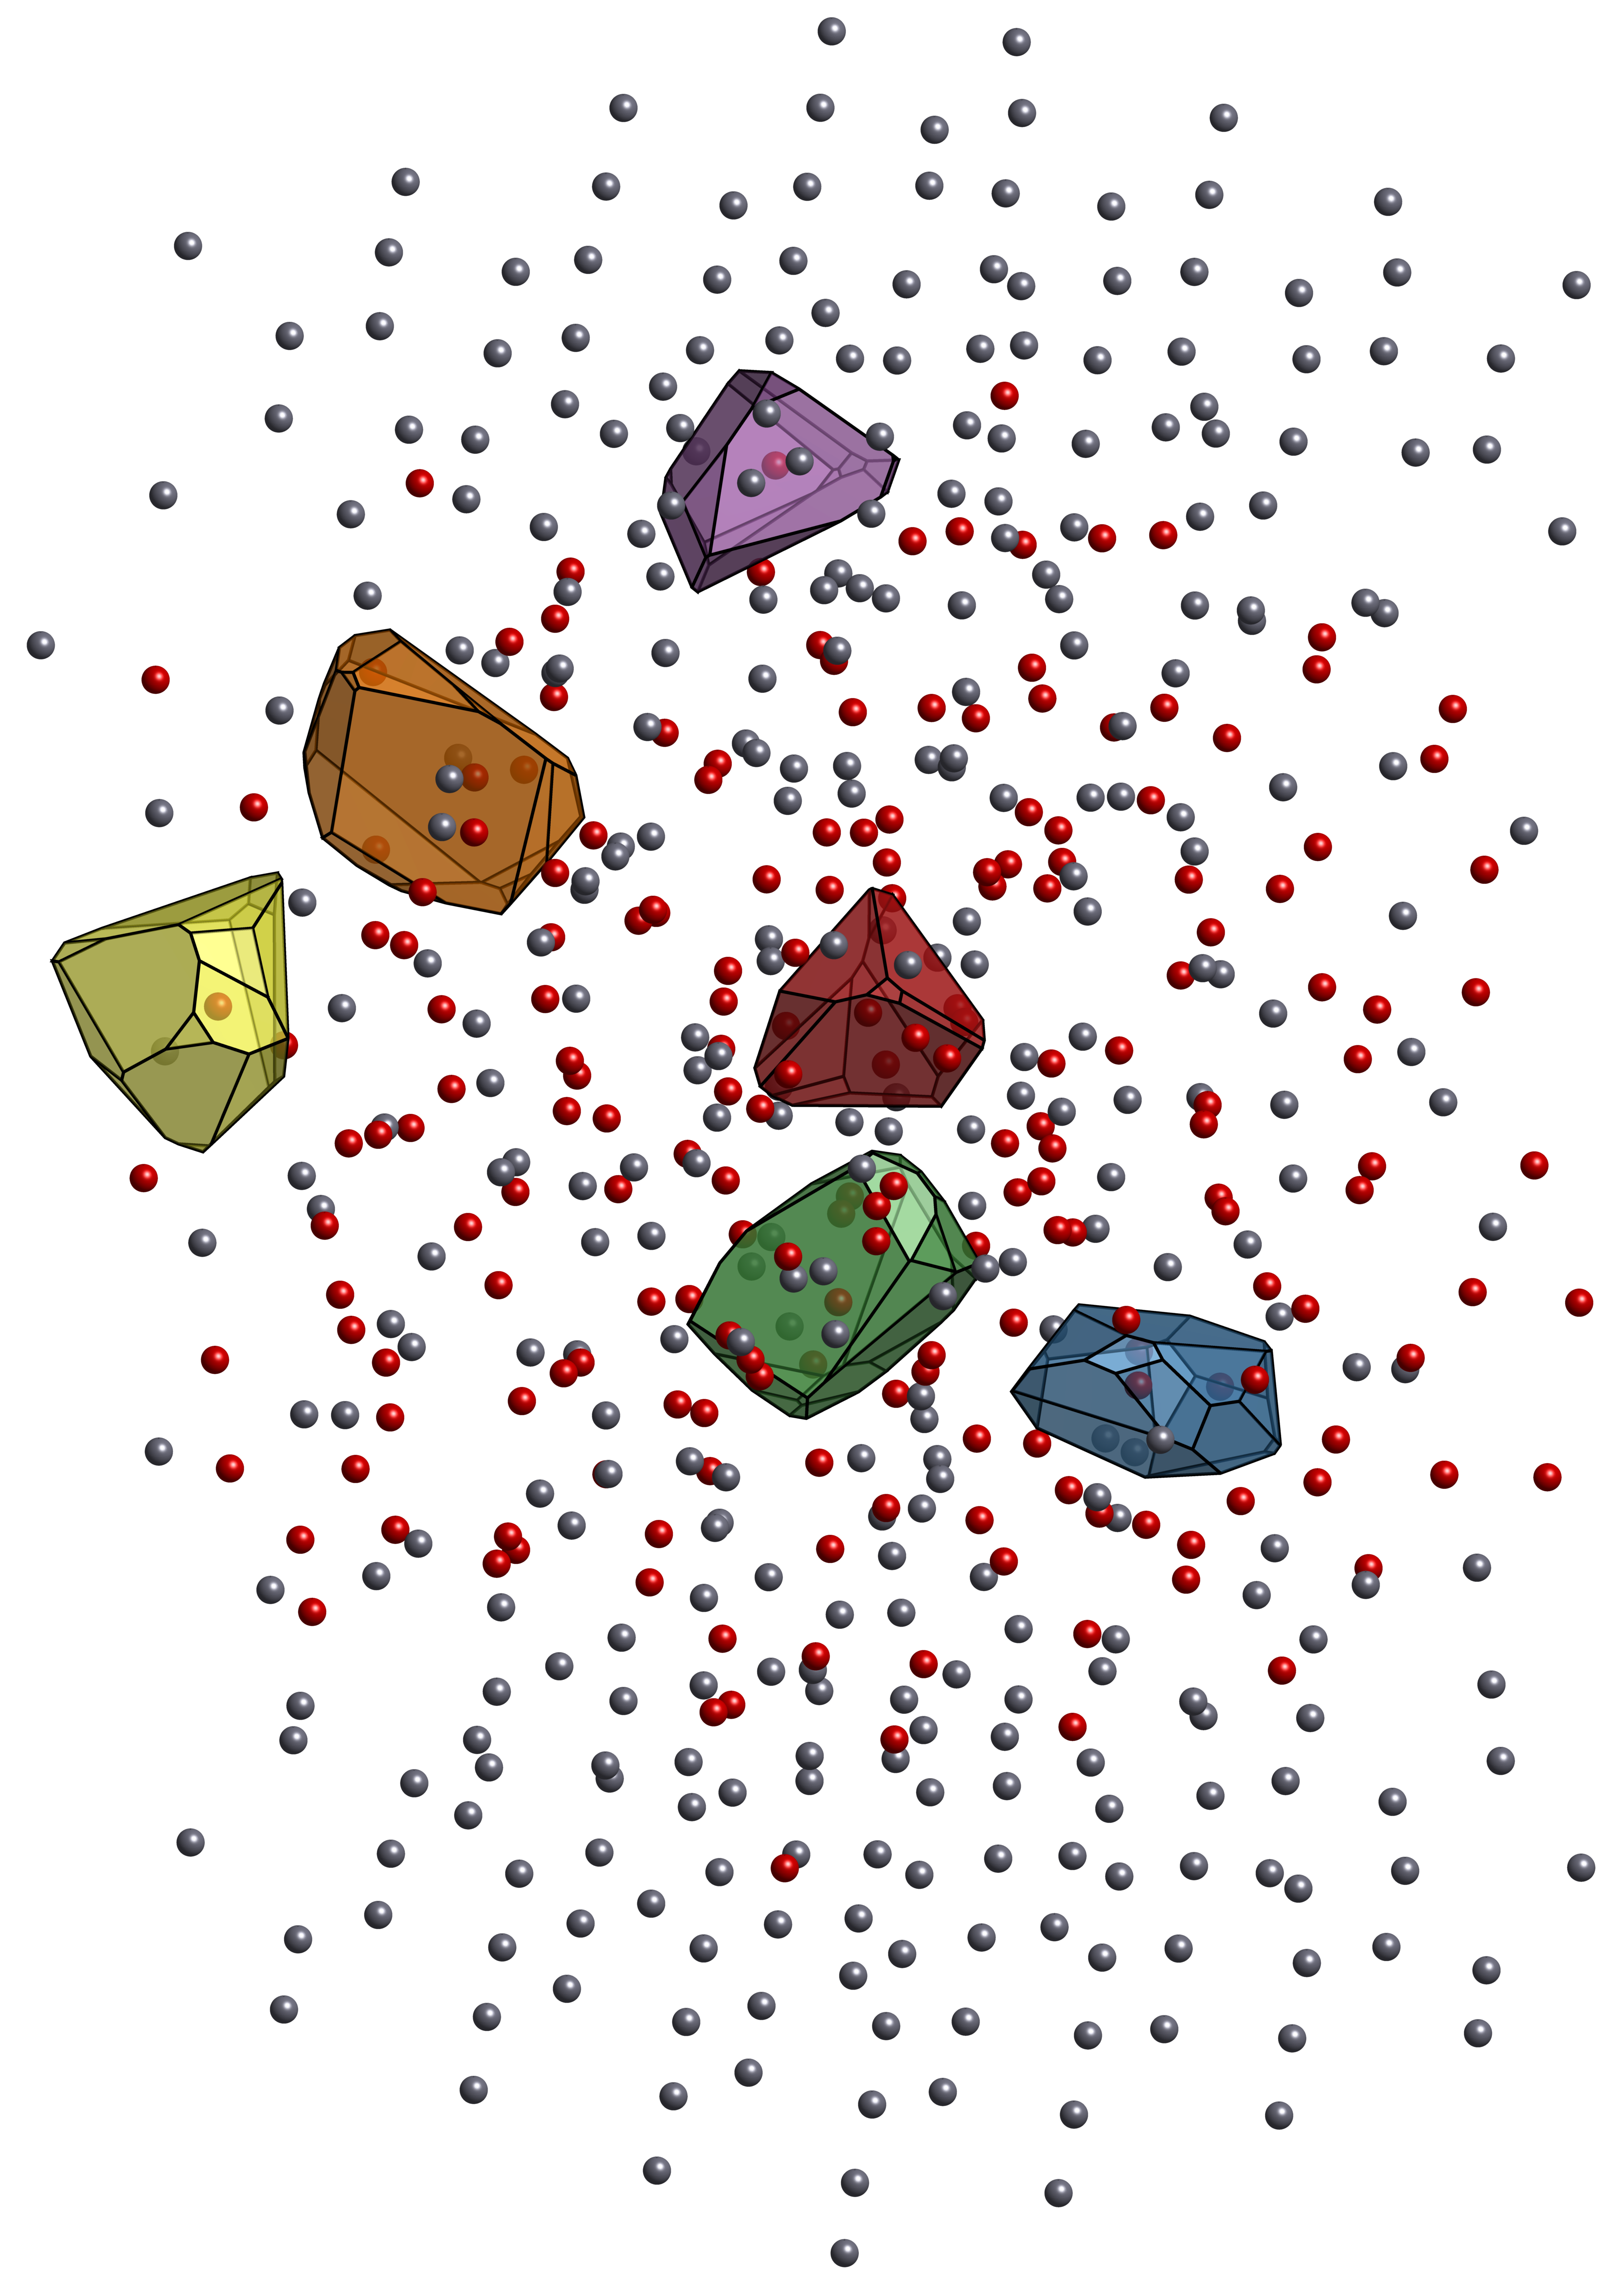
\includegraphics{vors}};

%Layouts
%SBS Underneath
%[yscale=3,xshift=-5cm,yshift=-5.25cm]
%[yscale=3,xshift=5cm,yshift=-5.25cm]
%[yscale=3,xshift=-5cm,yshift=-6.75cm]
%[yscale=3,xshift=5cm,yshift=-6.75cm]
%[yscale=3,xshift=-5cm,yshift=-8.25cm]
%[yscale=3,xshift=5cm,yshift=-8.25cm]

%Right Stack
%[yscale=3,xshift=13cm,yshift=3cm]
%[yscale=3,xshift=13cm,yshift=1.6cm]
%[yscale=3,xshift=13cm,yshift=0.2cm]
%[yscale=3,xshift=13cm,yshift=-1.2cm]
%[yscale=3,xshift=13cm,yshift=-2.6cm]
%[yscale=3,xshift=13cm,yshift=-4cm]

%Left Stack
%Will be similar toabove but xshift will be arouns -11cm.
%choose left or right stack such that junction is in the margins.

\begin{scope}[yscale=3,xshift=13cm,yshift=3cm]
    %large3 (purple)
    \filldraw [black,fill=Set1-7-4,fill opacity=0.7] (-3.5,1.1) -- (-3,1.1) -- (-3,0.9) -- (-3.5,0.9) --cycle;
    \node at (-1.8,1) {\Large 6 \includegraphics[width=0.5em]{aluminium}\, 13 \includegraphics[width=0.5em]{oxygen}};
    \node at (-2.2,0.7) {\Large $\xi = 1.44$};
    \node at (-2.2,0.5) {\Large $\wp_x = -0.035$ \AA};
    \node at (-2.22,0.3) {\Large $\wp_y = \phantom{-}0.013$ \AA};
    \node at (-2.2,0.1) {\Large $\wp_z = \phantom{-}0.034$ \AA};

    \draw[level] (3,0) node[above=1.7em, right] {$E_{01} = 11.81$ THz} -- (0,0) node[left] {$E_{0}$};
    \draw[level] (3,0.414) node[above=0.6em, right] {$E_{12} = 4.97$ THz} -- (0,0.414) node[left] {$E_{1}$};
    \draw[level] (3,0.589) node[above=0.1em, right] {$E_{23} = 0.47$ THz} -- (0,0.589) node[below=0.4em, left] {$E_{2}$};
    \draw[level] (3,0.605) node[above=0.9em, right] {$E_{34} = 6.31$ THz} -- (0,0.605) node[above=0.4em, left] {$E_{3}$};
    \draw[level] (3,0.827) node[above=0.7em, right] {$E_{45} = 4.92$ THz} -- (0,0.827) node[left] {$E_{4}$};
    \draw[level] (3,1) -- (0,1) node[left] {$E_{5}$};
\end{scope}

\begin{scope}[yscale=3,xshift=13cm,yshift=1.6cm]
    %large4 (orange)
    \filldraw [black,fill=Set1-7-5,fill opacity=0.7] (-3.5,1.1) -- (-3,1.1) -- (-3,0.9) -- (-3.5,0.9) --cycle;
    \node at (-1.8,1) {\Large 9 \includegraphics[width=0.5em]{aluminium}\, 12 \includegraphics[width=0.5em]{oxygen}};
    \node at (-2.2,0.7) {\Large $\xi = 1.44$};
    \node at (-2.2,0.5) {\Large $\wp_x = -0.035$ \AA};
    \node at (-2.22,0.3) {\Large $\wp_y = \phantom{-}0.013$ \AA};
    \node at (-2.2,0.1) {\Large $\wp_z = \phantom{-}0.034$ \AA};

    \draw[level] (3,0) node[above=1.7em, right] {$E_{01} = 11.81$ THz} -- (0,0) node[left] {$E_{0}$};
    \draw[level] (3,0.414) node[above=0.6em, right] {$E_{12} = 4.97$ THz} -- (0,0.414) node[left] {$E_{1}$};
    \draw[level] (3,0.589) node[above=0.1em, right] {$E_{23} = 0.47$ THz} -- (0,0.589) node[below=0.4em, left] {$E_{2}$};
    \draw[level] (3,0.605) node[above=0.9em, right] {$E_{34} = 6.31$ THz} -- (0,0.605) node[above=0.4em, left] {$E_{3}$};
    \draw[level] (3,0.827) node[above=0.7em, right] {$E_{45} = 4.92$ THz} -- (0,0.827) node[left] {$E_{4}$};
    \draw[level] (3,1) -- (0,1) node[left] {$E_{5}$};
\end{scope}

\begin{scope}[yscale=3,xshift=13cm,yshift=0.2cm]
    %large5 (yellow)
    \filldraw [black,fill=Set1-7-6,fill opacity=0.7] (-3.5,1.1) -- (-3,1.1) -- (-3,0.9) -- (-3.5,0.9) --cycle;
    \node at (-1.8,1) {\Large 11 \includegraphics[width=0.5em]{aluminium}\, 13 \includegraphics[width=0.5em]{oxygen}};
    \node at (-2.2,0.7) {\Large $\xi = 1.44$};
    \node at (-2.2,0.5) {\Large $\wp_x = -0.035$ \AA};
    \node at (-2.22,0.3) {\Large $\wp_y = \phantom{-}0.013$ \AA};
    \node at (-2.2,0.1) {\Large $\wp_z = \phantom{-}0.034$ \AA};

    \draw[level] (3,0) node[above=1.7em, right] {$E_{01} = 11.81$ THz} -- (0,0) node[left] {$E_{0}$};
    \draw[level] (3,0.414) node[above=0.6em, right] {$E_{12} = 4.97$ THz} -- (0,0.414) node[left] {$E_{1}$};
    \draw[level] (3,0.589) node[above=0.1em, right] {$E_{23} = 0.47$ THz} -- (0,0.589) node[below=0.4em, left] {$E_{2}$};
    \draw[level] (3,0.605) node[above=0.9em, right] {$E_{34} = 6.31$ THz} -- (0,0.605) node[above=0.4em, left] {$E_{3}$};
    \draw[level] (3,0.827) node[above=0.7em, right] {$E_{45} = 4.92$ THz} -- (0,0.827) node[left] {$E_{4}$};
    \draw[level] (3,1) -- (0,1) node[left] {$E_{5}$};
\end{scope}

\begin{scope}[yscale=3,xshift=13cm,yshift=-1.2cm]
    %ASYM (RED) Complete
    \filldraw [black,fill=Set1-7-1,fill opacity=0.7] (-3.5,1.1) -- (-3,1.1) -- (-3,0.9) -- (-3.5,0.9) --cycle;
    \node at (-1.8,1) {\Large 5 \includegraphics[width=0.5em]{aluminium}\, 9 \includegraphics[width=0.5em]{oxygen}};
    \node at (-2.2,0.7) {\Large $\xi = 1.44$};
    \node at (-2.2,0.5) {\Large $\wp_x = -0.035$ \AA};
    \node at (-2.22,0.3) {\Large $\wp_y = \phantom{-}0.013$ \AA};
    \node at (-2.2,0.1) {\Large $\wp_z = \phantom{-}0.034$ \AA};

    \draw[level] (3,0) node[above=1.7em, right] {$E_{01} = 11.81$ THz} -- (0,0) node[left] {$E_{0}$};
    \draw[level] (3,0.414) node[above=0.6em, right] {$E_{12} = 4.97$ THz} -- (0,0.414) node[left] {$E_{1}$};
    \draw[level] (3,0.589) node[above=0.1em, right] {$E_{23} = 0.47$ THz} -- (0,0.589) node[below=0.4em, left] {$E_{2}$};
    \draw[level] (3,0.605) node[above=0.9em, right] {$E_{34} = 6.31$ THz} -- (0,0.605) node[above=0.4em, left] {$E_{3}$};
    \draw[level] (3,0.827) node[above=0.7em, right] {$E_{45} = 4.92$ THz} -- (0,0.827) node[left] {$E_{4}$};
    \draw[level] (3,1) -- (0,1) node[left] {$E_{5}$};
\end{scope}

\begin{scope}[yscale=3,xshift=13cm,yshift=-2.6cm]
    %large1 (green)
    \filldraw [black,fill=Set1-7-3,fill opacity=0.7] (-3.5,1.1) -- (-3,1.1) -- (-3,0.9) -- (-3.5,0.9) --cycle;
    \node at (-1.8,1) {\Large 8 \includegraphics[width=0.5em]{aluminium}\, 11 \includegraphics[width=0.5em]{oxygen}};
    \node at (-2.2,0.7) {\Large $\xi = 1.44$};
    \node at (-2.2,0.5) {\Large $\wp_x = -0.035$ \AA};
    \node at (-2.22,0.3) {\Large $\wp_y = \phantom{-}0.013$ \AA};
    \node at (-2.2,0.1) {\Large $\wp_z = \phantom{-}0.034$ \AA};

    \draw[level] (3,0) node[above=1.7em, right] {$E_{01} = 11.81$ THz} -- (0,0) node[left] {$E_{0}$};
    \draw[level] (3,0.414) node[above=0.6em, right] {$E_{12} = 4.97$ THz} -- (0,0.414) node[left] {$E_{1}$};
    \draw[level] (3,0.589) node[above=0.1em, right] {$E_{23} = 0.47$ THz} -- (0,0.589) node[below=0.4em, left] {$E_{2}$};
    \draw[level] (3,0.605) node[above=0.9em, right] {$E_{34} = 6.31$ THz} -- (0,0.605) node[above=0.4em, left] {$E_{3}$};
    \draw[level] (3,0.827) node[above=0.7em, right] {$E_{45} = 4.92$ THz} -- (0,0.827) node[left] {$E_{4}$};
    \draw[level] (3,1) -- (0,1) node[left] {$E_{5}$};
\end{scope}

\begin{scope}[yscale=3,xshift=13cm,yshift=-4cm]
    %large1 (blue)
    \filldraw [black,fill=Set1-7-2,fill opacity=0.7] (-3.5,1.1) -- (-3,1.1) -- (-3,0.9) -- (-3.5,0.9) --cycle;
    \node at (-1.8,1) {\Large 13 \includegraphics[width=0.5em]{aluminium}\, 5 \includegraphics[width=0.5em]{oxygen}};
    \node at (-2.2,0.7) {\Large $\xi = 1.44$};
    \node at (-2.2,0.5) {\Large $\wp_x = -0.035$ \AA};
    \node at (-2.22,0.3) {\Large $\wp_y = \phantom{-}0.013$ \AA};
    \node at (-2.2,0.1) {\Large $\wp_z = \phantom{-}0.034$ \AA};

    \draw[level] (3,0) node[above=1.7em, right] {$E_{01} = 11.81$ THz} -- (0,0) node[left] {$E_{0}$};
    \draw[level] (3,0.414) node[above=0.6em, right] {$E_{12} = 4.97$ THz} -- (0,0.414) node[left] {$E_{1}$};
    \draw[level] (3,0.589) node[above=0.1em, right] {$E_{23} = 0.47$ THz} -- (0,0.589) node[below=0.4em, left] {$E_{2}$};
    \draw[level] (3,0.605) node[above=0.9em, right] {$E_{34} = 6.31$ THz} -- (0,0.605) node[above=0.4em, left] {$E_{3}$};
    \draw[level] (3,0.827) node[above=0.7em, right] {$E_{45} = 4.92$ THz} -- (0,0.827) node[left] {$E_{4}$};
    \draw[level] (3,1) -- (0,1) node[left] {$E_{5}$};
\end{scope}

\end{tikzpicture}%
\end{document}

